\lstset{language=Java}

\section{\mt{Asztali kliens}{}}

\block{
	\subsection{\mt{Bevezetés}{}}

	\p{\mt{%
		Az asztali kliens az API könyvtár segítségével kommunikál az API szerverrel.
		A kliens a JavaFX felhasználói felület platformot használja.
		A fejlesztéshez a Netbeans IDE használható.
	}{}}
}

\block{
	\subsection{\mt{Asztali kliens osztályai}{}}
	
	\subsubsection{\mt{Worker osztály}{}}
	
	\p{\mt{%
		A \code{Worker} osztály a háttérben futó folyamatok kezeléséért felelős.
	}{}}
}

\block{
	\subsubsection{\mt{EasyInventoryDesktop osztály}{}}
	
	\p{\mt{%
		A program az \code{EasyInventoryDesktop} osztályban kezdődik, ahol a kezdő metódus betölti a nyelvfájlokat, beállítja az ablakot és elindítja a bejelentkezési felület létrehozását.
		Emellett ez az osztály állítja be az eseménykezelőket és hozza létre a bejelentkezés utáni felületet is.
	}{}}
}

\begin{landscape}
	\begin{figure}
		\centering
		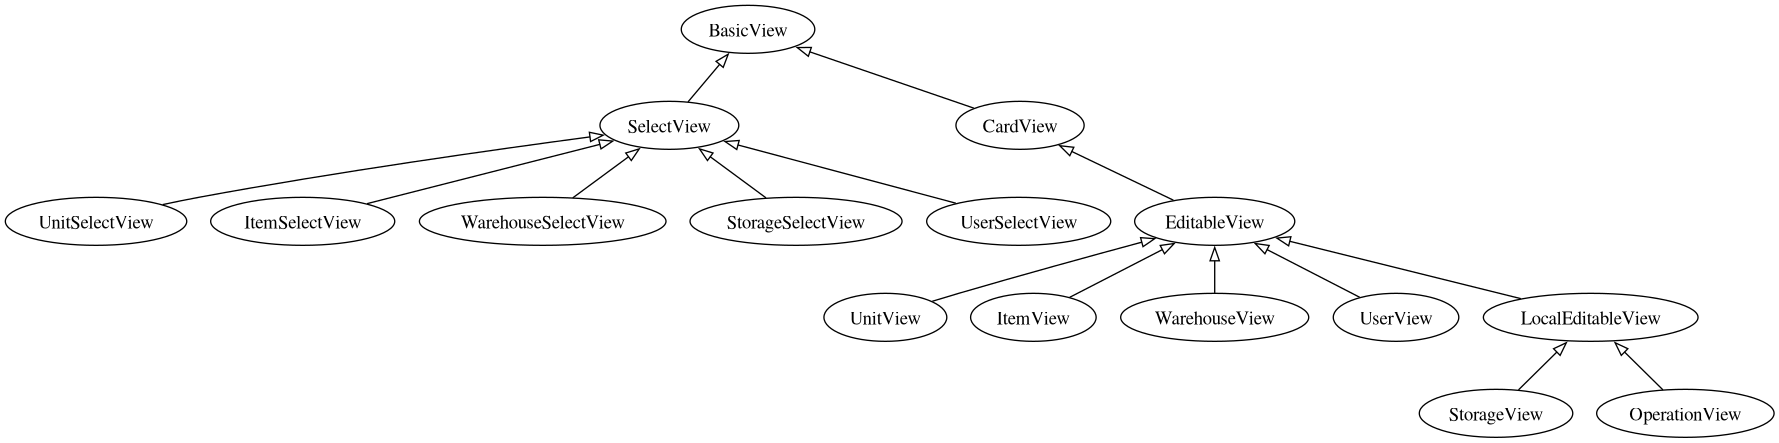
\includegraphics[width=\linewidth]{desktopclient.classes.png}
		\caption{\mt{Listázó osztályok diagrammja}{}}
	\end{figure}
\end{landscape}

\block{
	\subsubsection{\mt{BasicView osztály}{}}
	
	\p{\mt{%
		A \code{BasicView} absztrakt osztály a különböző listázási felületek szülőosztálya.
		Ez kezeli a listázáshoz tartozó újratöltés, keresés és pagináció menüelemeket.
		A \code{reload} funkció betölti a lista elemeit a megadott paraméterek alapján (keresési szöveg,kezdő pozíció,mennyiség és archivált-e).
		Ezt a funkciót a \code{Worker} szála hívja meg.
		A \code{createEntry} funkció feladata, hogy vizualizálja a betöltött adatokat.
	}{}}
}

\block{
	\subsubsection{\mt{SelectView osztály}{}}
	
	\p{\mt{%
		A \code{SelectView} absztrakt osztály a különböző kiválasztási felületek szülőosztálya.
		Ez az osztály implementálja a \code{createEntry} funkciót, amely a \code{showInfo} meghívásáért felel, amely vizualizálja a betöltött adatot.
		A \code{showInfo} -nak nem kell kiválasztás gombot hozzáadnia, mivel azt a \code{createEntry} megteszi helyette.
	}{}}
}

\block{
	\subsubsection{\mt{CardView osztály}{}}
	
	\p{\mt{%
		A \code{CardView} absztrakt osztály olyan listázási felületek szülőosztálya amelyek káryákban jelenítik meg az adatokat.
		A \code{createActionButtons} funkció feladata a akció gombot létrehozása.
		A \code{getArchivalUnixtime} funkció feladata az archiválás idejének visszaadása, \code{Long.MAX\_VALUE} ha nem archivált.
		A \code{showInfo} funkció feladata, hogy vizualizálja az adatot a kártyán belül.
	}{}}
}

\block{
	\subsubsection{\mt{EditableView osztály}{}}
	
	\p{\mt{%
		A \code{EditableView} absztrakt osztály a \code{CardView} osztályt szerkesztési gombokkal egészíti ki.
		Ez implementálja a \code{createActionButtons} funkciót szerkesztés és törlés gomb létrehozásával.
		A \code{showDialog} funkció feladata a szerkesztési és létrehozási dialógus létrehozása.
		A \code{delete} funkció feladata az adat törlése.
	}{}}
}

\block{
	\subsubsection{\mt{LocalEditableView osztály}{}}
	
	\p{\mt{%
		A \code{LocalEditableView} absztrakt osztály a \code{EditableView} osztályt telephely kiválasztási menüvel egészíti ki.
	}{}}
}

\begin{landscape}
	\begin{figure}
		\centering
		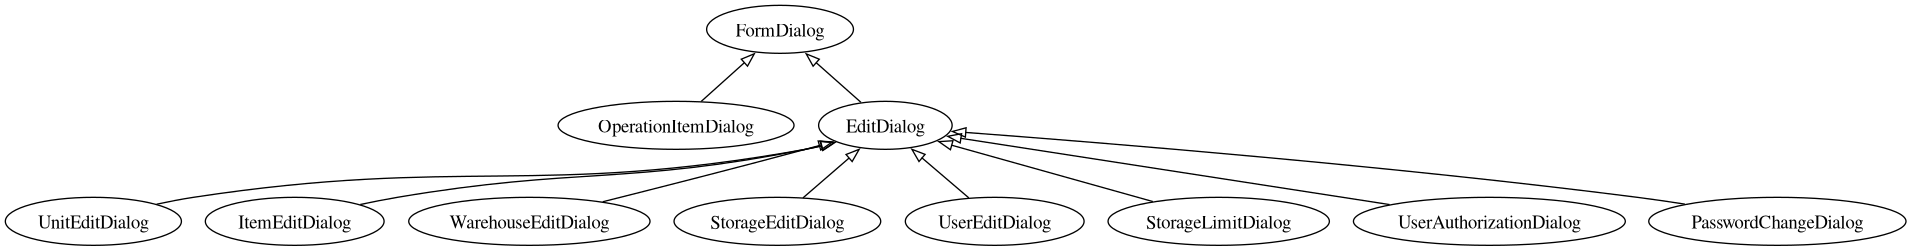
\includegraphics[width=\linewidth]{desktopclient.classes2.png}
		\caption{\mt{Dalógus osztályok diagrammja}{}}
	\end{figure}
\end{landscape}

\block{
	\subsubsection{\mt{FormDialog osztály}{}}
	
	\p{\mt{%
		A \code{FormDialog} absztrakt osztály a bemeneti felügró ablakok szülőosztálya.
		A \code{createEditFields} funkció a bemenetek lérhehozásáért felelős.
		Az \code{applyEdits} funkciő a bemenet értelmezéséért felelős.
	}{}}
}

\block{
	\subsubsection{\mt{EditDialog osztály}{}}
	
	\p{\mt{%
		Az \code{EditDialog} absztrakt osztály a \code{FormDialog} osztályt mentéssel egészíti ki.
	}{}}
}



